%\documentclass[11pt]{AdvInfo}
\documentclass[11pt,a4paper]{article}
\usepackage{graphicx}
\usepackage[T2A,T1]{fontenc}
\usepackage[utf8]{inputenc}
\usepackage[russian, UKenglish]{babel}
\usepackage{quotes}
\usepackage[hyphens]{url}
%\usepackage{hyperref}  
\usepackage{setspace}
\pagenumbering{arabic}
\newcommand{\mycaption}[1]{
  \centerline{\parbox{11cm}{\vspace{0.25cm}{\caption{\small#1}}}}
}

\begin{document}

%***********************************************************************
% TITLE PAGE
%***********************************************************************
\begin{titlepage}
\begin{large}
\begin{center}

\textbf{Leipzig University}\\[5pt]
Faculty of Mathematics and Computer Science \\


\vskip 4cm

{\Large \textbf{Schematisation in the Work of G.P. Shchedrovitsky}}
\vskip 0.3cm
Research Seminar "Sustainability, Environment, Management"

\vfill

\textbf{Marvin M\"uller}\\[6pt]
Matriculation Number: 3786960\\
Contact: ja25opir@studserv.uni-leipzig.de\\

\vskip 1cm

\today
\end{center}

\end{large}
\end{titlepage}
\newpage

%***********************************************************************
% ABSTRACT
%***********************************************************************

%\thispagestyle{empty}
%\begin{abstract}
%\end{abstract}
%\newpage

%***********************************************************************
% ToC
%***********************************************************************

\thispagestyle{empty}
\tableofcontents
\newpage

%***********************************************************************
% CONTENT
%***********************************************************************

\section{Introduction}

Business Process Modelling is an essential tool that enables the analysis, improvement and automation of activities within an enterprise by describing their properties, such as dependencies and objectives \cite[p. 129ff.]{AguilarSavn2004}. While this kind of verbalisation and abstraction is important for intra-business management it also allows comparison between businesses. \\
Although this kind of modelling and theory building are of crucial importance, there is a large amount of modelling that often does not play a role in practice. Therefore a framework or instruction for theory building itself is needed. The concepts introduced by the Russian philosopher G. P. Shchedrovitsky and his methodological movement work on exactly that. His theories were tested in several action games he directed, which took place from the 1980s to the post-Soviet period. \\
This paper will give a brief overview over Shchedrovitsky's biography, his work on the concept of managerial activity and the notion of schematisation. Furthermore the impact of informal practices of management on the transformation of the Soviet Union is outlined and the Organisational-Activity Games invented by Shchedrovitsky are presented.
%TODO Inhalte nochmal checken (vorhergehender Satz)
%TODO Rechtschreibung prüfen (Google)
%TODO todo's checken


\section{Biography of G.P. Shchedrovitsky}

Georgy Petrovich Shchedrovitsky (in Cyrillic: \foreignlanguage{russian}{Георгий Петрович Щедровицкий}) was born in Moscow on 23 February 1929 \cite[p. 1]{Davydova}. His mother was a microbiologist while his father was an engineer in the Soviet aviation industry and later became director of a research institute for the aviation industry, Orgaviaprom. He grew up in privileged surroundings and had daily interactions with members of the Communist Party of the Soviet Union and the military industry \cite[p. 7]{Rindzeviit2015}. Thus he was able to understand at an early stage how power was interwined in the Soviet Union and could make important contacts. \\
Shchedrovitsky began to study at the Faculty of Philosophy of Moscow State University in 1949 after studying three years of physics. In this time he already began to work on topics like the methodology of science and the theory of thinking \cite[p. 1]{Davydova}. Before graduating with honours in 1953 he began working as a school teacher in 1951. The subjects he taught until 1958 were logic, psychology and physics \cite[p. 1]{Davydova} $/$ \linebreak \cite[p. 7]{Rindzeviit2015}. \\
In 1957 Shchedrovitsky published his first scientific articles with the topics thinking activity and problems of thinking \cite[p. 1]{Davydova}. While he continued to publish articles and started to work in the APN RSFS publishing house in 1958, he became widely known for his seminars which he first held in 1955. They had different topics like "the complex and systematic study of thinking" \cite[p. 1]{Davydova}, "structural-system analysis methods in science and technology" \cite[p. 2]{Davydova} and "problems of physical culture and sports" \cite[p. 4]{Davydova} and mostly belonged to the fields of methodology and theory of thinking. \\
Through his fascination for philosophy and logic and the interconnections between humanities and mathematical sciences in the 1950s and 1960s he made the acquaintance with many future prominent Russian thinkers from across different fields of science. During this time the "so‑called Moscow methodological circle [...] originated as an informal gathering of logic students in a pub on Gor’kii street" \cite[p. 7]{Rindzeviit2015} which was led by Shchedrovitsky since 1954. The circle mainly focussed on the systems approach and furthermore the strategic fields of cybernetics and organised seminars which were attended mostly by young scholars \cite[p. 8]{Rindzeviit2015}. In one of these seminars they "discussed Western approaches to general systems theory" [Ibid.] which was one of the reasons why the group attracted the attention of the KGB. However, their meetings were not banned as most of the topics they covered were innovative and also promoted in the Soviet Union. Nevertheless, he was expelled from the Communist Party of the Soviet Union in 1968 after signing a letter to the leaders of the CPSU in defence of Aleksander Ginzburg and Iurii Galanskov, who were accused of dissidence. Thanks to his contacts he could continue his research work and was able to earn money "at the experimental workshop of the All‑Union of Artists" \cite[p. 8]{Rindzeviit2015} and as an employee e.g. at sports research institutes. Shchedrovitsky was refused to work at the biggest Soviet institutes "where much of the innovative research into systems approach and forecasting was concentrated" [Ibid.] but kept in touch with people from these circles. Thus his work could find recognition in the highest circles of Soviet managers, although his underground seminars and informal clubs were always viewed with distrust by the Soviet political leadership \cite[p. 9]{Rindzeviit2015}.  In most non-russian scholarly works on the history of Soviet governance, Shchedrovitsky is not mentioned. The reason may be that he had no stable affiliation and operated under the umbrella of different institutes. Acting as an independent contractor did not fit into the framework of the Gosplan where institutes provided data and methods to the State Planning Committee which created and managed economic and social development plans centrally \cite[p. 7]{Rindzeviit2015}. \\
In Shchedrovitsky’s personal research the activity theory became a main target and he published articles concerning for example "bases for a general theory of activity, reflexion processes and their role in the development of activity" \cite[p. 3]{Davydova} and "the main conceptions of the activity theory and of the system approach" \cite[p. 4]{Davydova}. Between 1979 and 1991 he organised a series of so called Organisational-Activity Games, games that "aimed at handling certain concrete problems or situations" \cite{Naumov} and were based on a "new form of organising collective thinking and activity" \cite[p. 4]{Davydova}. These games played an important role in the transformation of economy and management in the Soviet Union that happened especially during the Perestroika period between 1985 and 1991. \\
Georgy Petrovich Shchedrovitsky died on 3 February 1994 in Bolshevo near Moscow.


\section{The transformation of management in the Soviet Union}

To get an impression of the impact and importance of Shchedrovitsky’s work it is essential to understand how management in terms of state planning was done in the Soviet Union and changed over time. \\ 
Dr Eglė Rindzevičiūtė, Associate Professor of Criminology and Sociology at Kingston University London, investigated studies that focus on the production mechanisms of Soviet future studies which were used to plan the further development of the Soviet Union. She states that these studies have very different ideas about the future which all together supported the actual way of transformation in and after the Soviet era. She also states that the production of futures deviating from the current path of the Soviet Union was "situated close to the centre of power" \cite[p. 1]{Rindzeviit2015} which made the transformation of the Soviet system "a transformation from within the system" [Ibid.].  

\subsection{Gosplan and goal-oriented governance}
Central institution of the Soviet planned economy was the Gosplan. Established in 1921 it was responsible for economic planning by creating plans in five year steps to control the economy. The planning was based on research by different scientific institutes such as the Council for the Study of Productive Forces or the Institute of Complex Transport Problems. Each institute collected data about the present and past for its respective topic and used it to make predictions about possible future developments \cite{Gosplan}. This research is comparable to future studies and is referred to as such by Rindzevičiūtė. \\
The introduction of scientific forecasting and the following development of a new interpretation of goal-oriented governance resulted in a change of the authoritarian Soviet government. "New tools promised better control of the future" \cite[p. 2]{Rindzeviit2015} but created "new spaces of action and new sources of authority" [Ibid.] which yielded a decrease of power of the Soviet regime. One of these tools was the methodology of management by Shchedrovitsky and his movement. But not all of the new actors and methods brought innovation but also plurality and uncertainty instead of stabilising visions. 

\subsection{De-formalisation of managerial relations}
The new way of distribution of power created informal relations. While such informal relations helped make the Soviet economy work, it "turned out to be a "modernisation trap" in the post‑Soviet context" \cite[p. 2]{Rindzeviit2015}. Rindzevičiūtė states that there is not enough knowledge about the real impact of these informal relations but notes that both formal and informal rules and practices work together in complex relations, as suggested by management theory, instead of contradicting each other. Thus, the soviet future was not only determined by "the official planning guidelines produced by the Party" \cite[p. 2]{Rindzeviit2015} but also influenced by "dispersed academic and management milieus, particularly among the policy sciences, such as global modelling and forecasting" [Ibid.]. \\
Shchdedrovitski’s approach can be interpreted as wanting to complement planning based on formal knowledge with informal practices in order to improve control over the future. Rindzevičiūtė defines formal knowledge as "[...] sciences produced within defined institutional environments, institutes and laboratories, documented in publications and fed to into the governmental process through reports and statistics ; in short, the end products of future expertise" \cite[p. 3]{Rindzeviit2015}. While high modernist states create their future plans based on these formale sciences, Shchdedrovitski’s maxim was to de-formalise managerial relations and enable the Soviet government apparatus to survive its upheaval. \\
Therefore his methodology also questions the previous approach of the Soviet government to make decisions on the basis of information provided by scientific forecasting which can be described as an "input-output model of predictive expertise" \cite[p. 4]{Rindzeviit2015}. "Shchedrovitskii’s core belief was that knowledge could be used as a performative instrument of governance. The notion of intellectual technology, for Shchedrovitskii and his followers, was therefore not merely an analytical concept, but an instrument of governance that they sought to develop" [Ibid.]. 

\subsection{The notion of teleological behaviour}
The goal-oriented governance of the Soviet Union can also be described with the notion of teleological behaviour, which was introduced by the US scientists Wiener, Rosenblueth and Bigelow in 1943. It theorises goal-oriented behaviour which in turn states that not the past but future goals determine the behaviour. For this, the future must be an anticipated state whilst the goal of teleological behaviour is to reach this anticipated state within a process. The present state of the process has to change until it matches the anticipated state. \\
Soviet state planning can be described as teleological behaviour which used cybernetics as a tool to reach communism as the anticipated state. The concept of cybernetics was defined by Wiener in 1948 and deals with the behaviour of dynamical systems. These systems have to be controlled by giving inputs and monitoring behavioural feedback that should be considered for the next inputs. This is often referred to as the art of steermanship \cite{Wiener}. \\
Since teleological behaviour is not only about processing information but about goal-setting, teleological behaviour of individuals in the Soviet economy like managers, collectives or companies undermines their subsumption to the Communist Party. Also problematic in complex systems such as states is that the anticipated goals "tend to change over the course of action" \cite[p. 5]{Rindzeviit2015}.  \\
For these reasons, this was not the ideal approach to realise the communist utopia.  \\
Nevertheless it was still utilised by the Soviet state planners. They had the pragmatism to change the communist future and enforce reforms. This was helpful or even necessary in order to enable expertise to predict future states of natural resources and their use rates in the World and the Soviet Union, the population growth of the Soviet Union and in the World and the creation of new technology. \\
This flexibility of the communist future on the one hand reduced the power of the Communist Party but on the other hand led to significant innovations as, for example, it made Shchedrovitski’s approach possible.


\section{The methodological approach and schematisation}
Methodology can be defined in various ways. Beer, for example, states that Methodology describes the theory of methods from a single discipline and the general theory of scientific methods as part of logic and philosophy \cite[p. 9]{Beer}. \\
Shchedrovitsky declares that "The essence of [Methodology] is the creation of methods and projects" \cite[p. 7]{Principles}. 

\subsection{Basic concepts of the Moscow Methodological Circle}
In general the idea of the MMC is to schematise systematic situations in a multi-position manner so that collective problem solving as multi-position organisation of practices is possible. This organisation consists of practitioners from different fields of science. In Methodological Seminars and Organisational-Activity Games this idea is implemented and tested \cite[p. 269ff.]{Maracha2018}. \\
To implement these ideas, Maracha describes four basic concepts from the approach of the MMC as requirements to thinking: \\
The first concept is holism and reflexivity in relation to the other approaches and types of thinking. This means that systems must be seen as a whole concept, not only as a composition of individual parts. In addition, different approaches, for example from different fields like science, technology or design, are taken into account. \\
The second concept is the practical orientation of the MMC, which means that thinking should take the form of organising processes to solve problems. \\
The third concept is reflectivity as a practical orientation of thinking to itself. It requires the ability to rethink and re-construct. \\
The last concept is the “methodological turn" from thinking about systems as objects to organizing, performing and reflecting the process of systems thinking in practice \cite[p. 270]{Maracha2018}. 

\subsection{The systemic approach}
The previously mentioned concept of a system can be defined as follows: "A \emph{system} is a \emph{delimited set of components}. Their interaction realises a \emph{qualitatively new function} (emergent function) and thus constitutes \emph{a new unified whole}" \cite[p. 2]{GraebeSystems}. \\
In the systemic approach reality is modelled by reducing it to the essentials in three dimensions which are depicted in figure 1. While the whole system (1) is isolated from the environment, specifications and interfaces allow inputs and outputs (illustrated as solid arrows) from and to the environment. A throughput is guaranteed and illustrated as a dotted arrow. This dimension seemingly contradicts the basic concept of holism of the MMC, because in the theory of holism no boundaries exist. However, it can be said that holism prevails within the system. Inside the system different components (2) exist whose behaviour can be controlled by inputs and outputs. Relations between components are reduced to causally essential relationships and are illustrated as dashed arrows (3). \\
Following the systemic approach a system can only function when its components are put together. \\
According to Shchedrovitsky all analysis in the field of systems should start from the systems movement, not from the systemic approach. He attaches importance to the term movement because “it brings together representatives of different professions (engineers, military, teachers, scientists, philosophers, mathematicians, organisers and managers), who have different means and styles of thinking, different values and points of view” \cite[p. 3] {Principles}.

\begin{figure}[h!]
\centering
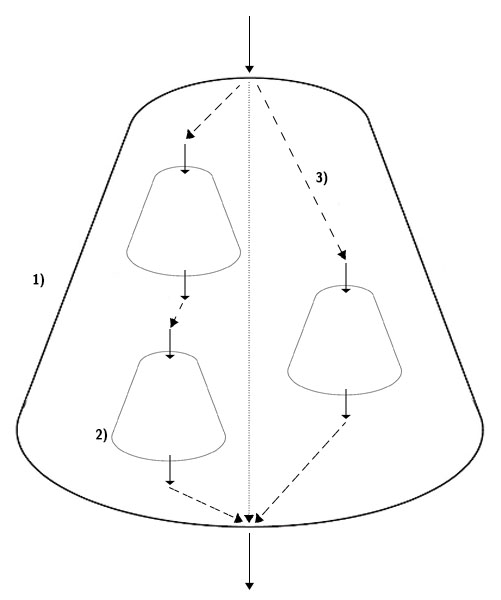
\includegraphics[scale=0.33]{fig_system.jpg}
\mycaption{Three reduction dimensions of a system}
\end{figure}

\subsection{Methodological School of Management}
The Methodological School of Management (MSM) is a collection of techniques, methods of work and rules of self-organisation based on the work of G. P. Shchedrovitsky gathered and completed with own concepts by V. B. Khristenko, A. G. Reus and A. P. Zinchenko. All of these three authors hold or held important posts in Russia. V. B. Khristenko was First Deputy Prime Minister of Russia from 1999 to 2000, Russian Minister of Industry and Energy from 2004 until 2007 and the Russian Minister of Industry and Trade from 2008 until 2012. He also was Chairman of the Board of the Eurasian Economic Commission from 2012 to 2016. A. G. Reus was Director of UIC Oboronprom, a holding company of the defence industry, from 2007 to 2012. From 2004 to 2007 he was Deputy Minister of Industry and Energy of the Russian Federation. A. P. Zinchenko was Head of the Management Department at the Togliatty Academy of Management. The MSM addresses organisers, leaders and managers \cite[p. 36]{MSM}. Preceding the introduction of the concept of schematisation are various concepts of the MSM.

\subsubsection{Activity and transformation}
The activity theory defined by Shchedrovitsky differs from the previously known naturalistic theory where the world consists of human subjects and objects. In Shchedrovitsky’s activity theory, based on the work of Vygotski, objects are secondary constructs whose nature depends on the activity applied to them. Furthermore, activity is a system that determines how individuals behave. \\
According to the MSM the world consists of elementary acts that are linked together. Moreover the world is organised by our consciousness that uses relationships that move outwards. When an activity takes place, a transformation also takes place: “We obtain some source material, capture it and apply to it certain actions, tools or equipment, in order to transform it into a particular product, meeting a goal. This product emerges from the act of activity. We use tools and equipment” \cite[p. 38]{MSM}. \\
Activities can be different from different perspectives due to different ways of consciousness. In the MSM the example of an excavator operator and the question if he or she is digging a ditch or operating the excavator is used. The answer is given as follows: when someone has learned how to operate the machine then he or she is digging a ditch \cite[p. 38f.]{MSM}. In this context private processual skills and knowledge are an important concept in machine-centred technology \cite[p. 6ff.]{GraebeTechnology} and is also referred to as an internalised tool in the MSM. \\
Figure 2 displays how the MSM imagines the relations between activities in an organisation. It consists of people within the framework of an organisation (comparable to a system or even component as shown in figure 1). The rectangle with the two arrows illustrates the “‘control panel’ of consciousness” \cite[p. 38ff.]{MSM} which represents that activities can be different from different perspectives as stated above. Activities can also be related and create links between people. For example, when someone’s work produces a product which is the source material for another person. The product can either be tools, equipment, or knowledge. The product of a leading person, as depicted in the top of the organisation, may not be a transformation of natural material but can organise the activity of other people. The leading person can influence other activities by changing goals, giving other knowledge and source material or by introducing new technology \cite[p. 38ff.]{MSM}. \\

\begin{figure}[h!]
\centering
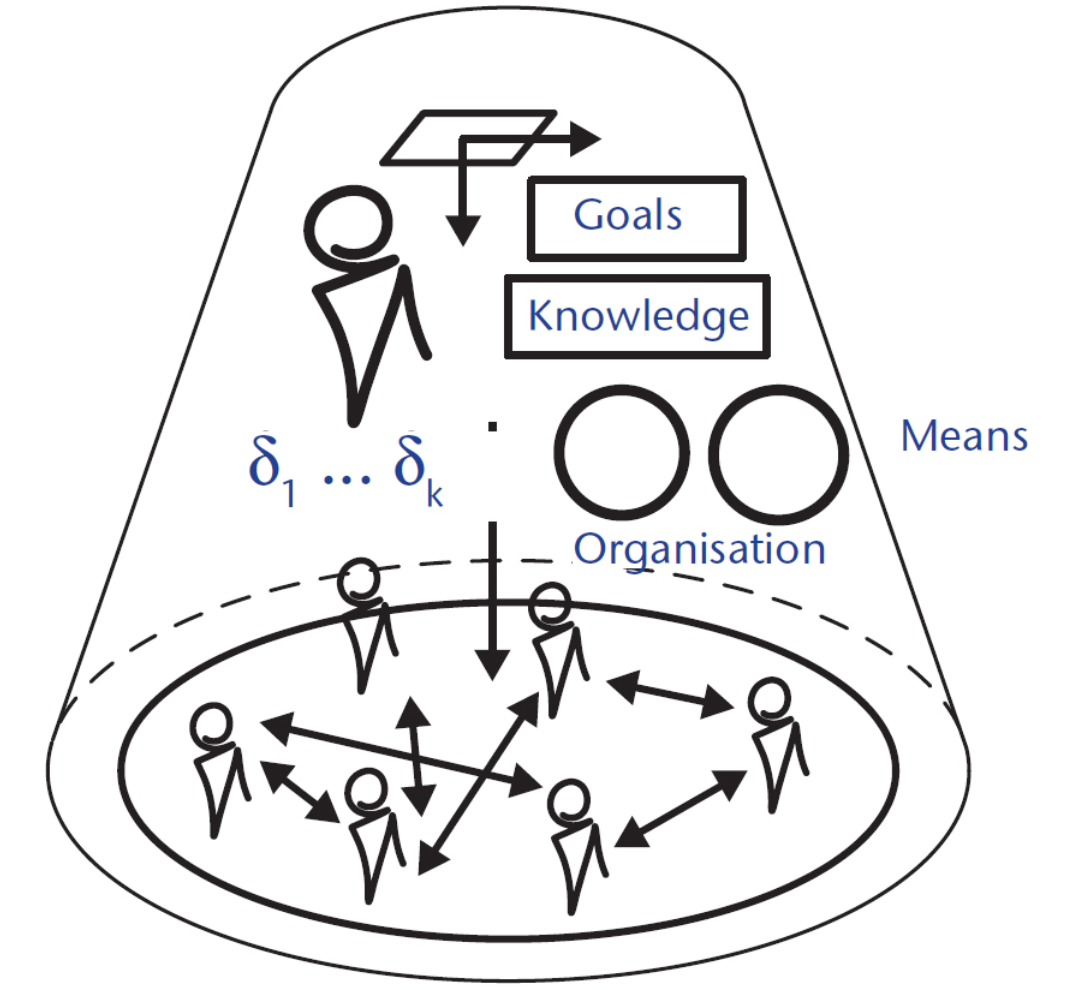
\includegraphics[scale=0.4]{fig_activity.png}
\mycaption{Activity management within an organisation \cite[p. 39]{MSM}}
\end{figure}

\subsubsection{Leadership and management}
For a more detailed view it is necessary to understand how Shchedrovitsky distinguishes between management and leadership. Management is only possible if objects have self-propulsion. Thus, management is applied to the process and not the objects. In contrast to this leadership affects only elements, mostly people, without self-propulsion. Furthermore it is only possible within a framework with organisational connections. The leading person sets the goals and objectives for other people in lower positions. They have to reject their own goals and objectives to accept those assigned to them. With that they also give up their self-propulsion and only move with the goals and objectives set by the leading person. However, in reality, people don’t give up their own goals and objectives completely but try to reach them within the performance of their official tasks. Hence self-propulsion begins and the need for management appears. This is the reason why leaders must both lead and manage \linebreak \cite[p. 51f.]{MSM}. \\
The leader or manager in figure 2 can perpetrate strategic management if the depicted organisation is an individual business area inside of a bigger strategic system consisting of several business areas. In other words the depicted organisation can be a component of a system as illustrated in figure 1. The relationships between all components of the system and with the system’s environment need to be organised to achieve strategic goals. Operational management focuses on design and development of an individual component, such as a business area.\cite[p. 1]{GraebeManagement}. 

\subsubsection{Organisation}
Shchedrovitsky states that organisers create the structure of a system or organisation such as a company. They chose the elements, people with internalised tools, and their locations and relations \cite[p. 51ff.]{MSM}.\\
The target of creating an organisation is to resolve management objectives. Only the organisers but not the organisation itself can have goals or objectives. That it has a purpose makes an organisation an artificial entity. From a natural viewpoint, other goals after the creation of an organisation may appear. The reason is the life of the people who work in the organisation as collectives. They tend to forget that the organisation was only created for the purpose to resolve specific goals \cite[p. 53f.]{MSM}. 

\subsubsection{The system-objective management scheme}
As stated in the penultimate paragraph, management requires self-propulsion of an object so that it passes from one state in another. Management-systems therefore exist in associations to the states of an object whose activity they manage. The object naturally passes from a state (1) to another (2) as illustrated in figure 3. For the existence of the management-system the object needs to pass into an artificial state (2’). Therefore the management-system must influence the object so that its original trajectory or activity is being transferred to an artificial-natural trajectory. The reason for this is that the management-system has a goal that matches state (2’) and therefore this is the desired state of the object to be managed. It also needs knowledge about the natural motion of the object, its own resources and if and how it can influence the trajectory of the object. Because the object gets captured and moved from the outside without self-propulsion, management is always aggressive \linebreak \cite[p. 54ff.]{MSM}. These concepts are similar to those of teleological behaviour as described in section 3.3.

\begin{figure}[h!]
\centering
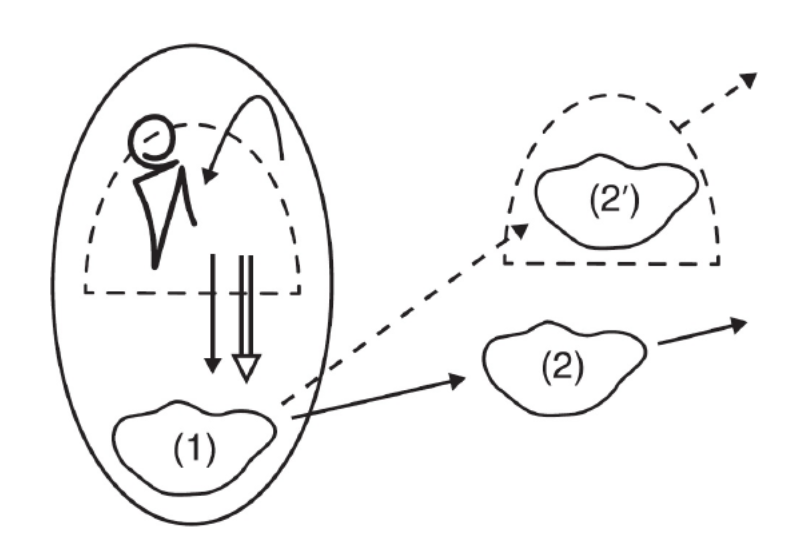
\includegraphics[scale=0.4]{fig_management.png}
\mycaption{A management-system applied to an object in different states \cite[p. 55]{MSM}}
\end{figure}


\subsubsection{Collective acting, reflexiveness, reality and practice of thinking}
According to the MSM, good organisers and leaders should sit in their offices and think instead of meeting other people frequently. \\
People always act in collectives with a minimum of three participants to solve a situation. In addition more collectives exist where people are in similar or different situations. These collectives interact with each other and boundaries between them can be very complex because most of the time situations cannot be clearly distinguished. \\
For the people that are part of those situations reflexiveness is an important concept. They need to see what they are doing and what is going on around them, e.g. what happens when they ask people from another situation a question. Furthermore complex tiers of reflexivity exist: people can think about what people in other situations think about what they are thinking. \\
While the world of mental activity is the real world, the world of thinking is the ideal world and “through the unification of pure thought with mental activity, a person always lives in these two worlds: the real world and the ideal world” \cite[p. 67]{MSM}. The real world is captured in different ideal mental schemes which are projections from the real world that differ because of various goals and objectives viewers can have. In this context thinking means to combine schemes like the drawings of positional people as done in the MSM, scientific laws or equations to see the real world through these representations of ideal worlds \cite[p. 56ff.]{MSM}. \\
The practice of thought means that practitioners are already thinking when they find themselves in real situations, as they are always thinking that they may have to switch into thinking mode. Before switching to it they put together schemes which they later take as starting points. Other posts they start from are the aforementioned concepts of practical mental activity and reflexivity \cite[p. 71]{MSM}.

\subsubsection{Problemisation and system analyses}
A problem or paradox in this context is defined as when two people say contrary things but both are right. To solve it, studying the object needs to be stopped and instead the modification of analysis concepts needs to start. \\
One of these paradoxes is the division of systems into subsystems in system analysis. While leaders of different business areas or components are tied to one leader in a higher position, they all lead or manage their own functioning systems. But according to the definition of the previously introduced systems approach a system cannot be divided into parts \cite[p. 78ff.]{MSM}.

\subsubsection{The administrative-organisational structure of places}
In another section the MSM states that principles have to deal with the \linebreak administrative-organisational structure of places. A system with people that constitute informally organised groups and relationships based on human attitudes like sympathy and antipathy. Principles need to stay outside of the system to reconstruct it so that it suits their purposes. This is done in an aggressive way as described in the definition of management before. Nevertheless it can be done with awareness \linebreak \cite[p. 82]{MSM}.

\subsection{Schematisation}
A schema is the depiction of the procedures, which are often wired like a network, applied to an object and not of the object itself. For schematisation images have to be created that need to differ from the depicted object. Otherwise the object itself could be used which would cancel the effect of schematisation. The image needs to correspond to the nature of work that wants to be done with it and must be suitable for construction and needs to be operable. In the MSM this is explained with the following example: formerly numbers were represented by sticks so that, for example, figure 10 was represented by ten sticks. This wasn’t suitable for an efficient way of counting nor applying arithmetic operations on, for example, 100 sticks. The operational and constructive abilities of these images were limited. For that reason the number ten was denoted by a new sign that the decimal system is based on \cite[p. 110f.]{MSM}. \\
According to Shchedrovitsky in schematisation it is important what the object of the analysis is and what is done when thoughts start being formulated. The latter was dealt with in section 4.3.5 as the practice of thought was discussed. Furthermore the “actions of an organiser, leader and manager consist in applying specific schemes to reality” \cite[p. 83.]{MSM} which was part of the reality of thinking reviewed also in section 4.3.5. Another important aspect is that the object structure depends on the chosen schemes, which can also be called the art of schematisation discussed in the first paragraph of section 4.4 [Ibid.].

\singlespacing
\noindent The ideas of the Moscow Methodological Circle and concepts from the Methodological School of Management were tested and examined in the Organisational-Activity Games. 


\section{Organisational-Activity Games}
According to S. B. Naumov Organisational-Activity Games (OAGs) “are development games, as opposed to brainstorms or role-playing games usually aimed at handling certain concrete problems or situations” \cite{Naumov}. \\
The basis of an OAG is a, mostly regional, problem that cannot be resolved with the current prevailing potential. The participants should be from different fields of science because most problems involve several disciplines and one concept of the process during the game was to review them from different perspectives which matches the general idea of the MMC described in section 4.1. Furthermore, participants should not just be theoreticians but also organisers, engineers, developers and other practicians. The field of participants is to be completed with methodologists and game technicians. An important game rule that Naumov emphasises is that whenever players suggest something they have to do it themselves to maintain the practical character of the game \cite{Naumov}.
 
\subsection{Procedure of an OAG}
Rindzevičiūtė claims that “Shchedrovitskii’s workshops, through which he disseminated his ideas among practitioners, are never described in detail, for these workshops were confidential in their character” \cite[p. 4]{Rindzeviit2015}. Luckily there is a more detailed report of the American professor C. ZumBrunnen who together with C. Miller were the first non-Soviets to participate in an OAG \cite[p. 1]{Brunnen}. Both got invited by the fellow geographer and friend of ZumBrunnen A. Mrost to attend to OAG "Analysis of the Prospective Development of the Orenburg Region under the Conditions of Self-Management and Self-Financing" which was held between November 25 and December 2 in 1989. Organisers of this OAG were S. V. Popov, president of the Inter-regional Methodological Association in Russia and mathematical oceanographer and G. P. Shchedrovitsky. \\
Before the game Popov described the Soviet system “as a "sticky tape" onto which all individual members of Soviet society had "become stuck" \cite[p. 3]{Brunnen} and that the "tape supposedly drained Soviet peoples of their individuality, their initiative, their ability to articulate their values and interests, their self- esteem, and their capacity for individual as well as collective innovative problem solving and decision-making” [Ibid.]. In the words of ZumBrunnen, Popov and Shchedrovitsky tried to overcome these obstacles and “"civilize their country" and to facilitate fundamental reform” \linebreak \cite[p. 2]{Brunnen}. \\
The OAG described by ZumBrunnen was sponsored by the local Communist Party which supports the thesis of the flexible communist future as described in section 3.3 and that the Soviet transformation came from the inside as stated in section 3. While some of the OAGs may just have been held to do something innovative without producing something just to further the perestroika, some created concrete results such as the selection of new factory managers or the creation of “stock-holding, joint-venture organizational firms between private coops and state enterprises” in Orenburg \linebreak \cite[p. 4]{Brunnen}. \\
Not only ZumBrunnen and Miller attended the OAG but in total 160 participants. 120 of them, party members, elected officials, workers, professionals etc., were representing the Orenburg region but mostly the local decision-making power structure. The other 40 participants were from similar organisations but other regions. \\
At the beginning of the game a briefing of the local conditions from different perspectives was done. Further Popov was presenting the goals and objectives of the game but not the players agenda. In this way they needed to encourage their individual and collective abilities of self-determination. The first two days were mostly spent with the concepts of self-management and -financing of local authorities \linebreak \cite[p. 4]{Brunnen}. Every morning the game started with a "reflective analysis of the situation in the game" [Ibid.] in small groups. Some of the time in the morning was also spent with game-technicians to think about what every player could take away from this unique experience for his or her own profession \cite[p. 5]{Brunnen}. After lunch and in the late evening a plenary meeting was held where every group reported and discussed their elaborations. During this the methodologists were confrontational, “producing some absolutely fascinating and highly charged exchanges” \cite[p. 4]{Brunnen}. From the first two days two processes emerged: "Conditions of the Region and the Possibility of Its Development" and "Critical Analysis of the Approaches to the Problems of Development in the Oblast" \cite[p. 5]{Brunnen}. During the whole game the players got confronted with the reality of their daily lives in several new ways during energised debates about the daily themes of the game. ZumBrunnen describes a heated exchange between Popov and a leader of the Young Communist League in Orenburg during the second day as a turning point of the game. While Popov provoked the player by badmouthing the Congress of People's Deputies the young man defended it as he was a just elected member of the Congress. During this discussion the other players recognised their own public masks and that they didn’t act in sense of their own values but only in complicity with the existing system. After that Popov disbanded all groups and said that the players were now ready to form their own groups as an act of self-determination \cite[p. 6]{Brunnen}. Groups that could formulate their own values and objectives the best were the winners of the game. \\
Shchedrovitsky said at a banquet held after the end of the game: “[...] we are not here by any process of self-determination. We are here because of the roles we play in this region or in this game” \cite[p. 6]{Brunnen}. So to speak, the OAGs were not to undermine the power of the Communist Party nor to establish capitalist reforms in the Soviet Union but to civilise and transform the country with innovations and new ways of thinking detached from any political systems.

\subsection{V. B. Khristenko's experiences with OAGs}
Another field report about Organisational-Activity Games is given by V. B. Khristenko in the MSM. The first OAG he participated in took place in the year 1988 when he was the junior manager at the Chelyabinsk Tractor Plant  \cite[p. 437ff.]{MSM}. Two years before the Perestroika period started and industrial, economic and social infrastructures in the Soviet Union were breaking down. As many others Khristenko saw his chance to be part of the radical change and registered himself for the OAG which was called "The development of a region within the framework of the development of a town" [Ibid.].\\
This OAG led to several suggestions the author proposed to the director of the tractor plant, e.g.:
\begin{itemize}
	\setlength\itemsep{0em}
	\item old-school methods (12-hour shifts, extra work shifts, shouting at staff) should be abolished
	\item the plant should be independent and allowed to keep the ownership of the manufactured products
	\item new organisation concept: production association, corporation, concern or a consortium
	\item move away from the idea of "production for the sake of production" to an idea that we need to meet the demands created by a marketing system
\end{itemize}
According to Khristenko thanks to the OAG "these ideas had been well thought out, well put together and well formulated" \cite[p. 441]{MSM}. After that he participated in many other OAGs during the Perestroika period, e.g.:
\begin{itemize}
	\setlength\itemsep{0em}
	\item "Ways of developing and raising the efficiency of the servicing of Kamaz Trucks for the national economy" (11 - 18 November 1988)
	\item "Prospects and programmes for the development of automobile manufacturing in the USSR" (16 - 24 December 1989)
	\item "A programme for the regional development of the city of Chelyabinsk and the Chelyabinsk Region" (26 November - 3 December 1990)
\end{itemize}

\section{Conclusion}
One of the core concepts of Shchedrovitsky‘s work is that knowledge and intellectual technology are instruments of governance. His own work became an important instrument during the transformation of the Soviet Union from the late 1970s to the post-Soviet era. While the conventional Soviet way of economy and state planning was the cybernetic notion of teleology where the key condition for control was reflexive goal setting, Shchedrovitsky‘s approach was the individual goal setting by individual managers. In conjunction with this theory of self-management is the concept of schematisation that determines how to organise, perform, reflect and also manage processes within a system. While schematisation is based on the systemic approach it makes a turn from thinking about objects to thinking about processes. The art of schematisation consists of the theories of activity, transformation, ways of consciousness, management, leadership, organisation, reflexiveness, pure thinking and some more additional concepts. The aforementioned were shortly explained in this paper to give a better understanding of how schematisation is done. \\
While Shchedrovitsky theoretically defined a new way of thinking about systems and processes he also could prove the feasibility and power of his thesis in hundreds of training events with mostly 150 to 200 participants that directly influenced the conversion of the Soviet economy \cite[p. 3]{Rindzeviit2015}. \\
Not only the success of his seminars and Organisational-Activity Games show the significance of his theses. Also many officials in high positions as V. B. Khristenko, A. G. Reus, A. P. Zinchenko, his son Petr Shchedrovitsky, who occupied the position of the Director‑General for Strategy at the Russian nuclear authority Rosatom and Russia's president Wladimir Putin are followers of his ideas. Thus, even almost 30 years after his death, they have not lost their significance. 

\newpage

% ****************************************************************************
% BIBLIOGRAPHY AREA
% ****************************************************************************

\thispagestyle{empty}
\bibliographystyle{unsrt}
\begin{thebibliography}{10}

\bibitem{AguilarSavn2004}
R.~S. Aguilar-Sav{\'{e}}n.
\newblock Business process modelling: Review and framework.
\newblock {\em International Journal of Production Economics}, 90(2):129--149,
  July 2004.

\bibitem{Davydova}
G.~A.~Davydova{,} translated~by H.~G.~Gräbe.
\newblock Biography of {G}. {P}. {S}hchedrovitsky.
\newblock December 2021.

\bibitem{Rindzeviit2015}
E.~Rindzevi{\v{c}}i{\={u}}t{\.{e}}.
\newblock The future as an intellectual technology in the soviet union.
\newblock {\em Cahiers du monde russe}, 56(1):111--134, January 2015.

\bibitem{Naumov}
S.~B.~Naumov{,} translated~by M.~Chumakin.
\newblock Organizational-activity games.
\newblock {\em Nature (Priroda)}, 4, 1987.

\bibitem{Gosplan}
The Gale~Group{,} Inc.
\newblock Gosplan.
\newblock {\em The Great Soviet Encyclopedia}, 1979.
\newblock \url{https://encyclopedia2.thefreedictionary.com/Gosplan}, Accessed:
  2022-03-29.

\bibitem{Wiener}
N.~Wiener.
\newblock Cybernetics.
\newblock {\em Scientific American}, 179(5):14--19, 1948.

\bibitem{Beer}
B.~Beer.
\newblock „methode“, „methodik“ und „methodologie“ in der
  ethnologie.
\newblock {\em EthnoScripts}, October 2008.

\bibitem{Principles}
G.~P.~Shchedrovitsky{,} translated~by H.~G.~Gräbe.
\newblock Principles and general scheme of the methodological organization of
  system-structural research and development.
\newblock 1981.

\bibitem{Maracha2018}
V.~Maracha.
\newblock Systems thinking and collective problem solving practices.
\newblock In {\em System analysis in economics {\textendash} 2018: Proceedings
  of the V International research and practice conference{\textendash}biennale
  (21{\textendash}23 november 2018)}. Prometheus publishing house, 2018.

\bibitem{GraebeSystems}
H.~G. Gräbe.
\newblock Systems and their development.
\newblock {\em Modelling Sustainable Systems and Semantic Web}, October 2021.

\bibitem{MSM}
V.~B. Khristenko{,} A. G. Reus{,} A.~P. Zinchenko.
\newblock {\em Methodological School of Management}.
\newblock Bloomsbury Information, July 2014.

\bibitem{GraebeTechnology}
H.~G. Gräbe.
\newblock Technology.
\newblock {\em Modelling Sustainable Systems and Semantic Web}, October 2021.

\bibitem{GraebeManagement}
H.~G. Gräbe.
\newblock {Supply Chains and SCOR – the Supply Chain Operations Reference
  Model}.
\newblock {\em Modelling Sustainable Systems and Semantic Web}, November 2021.

\bibitem{Brunnen}
C.~ZumBrunnen.
\newblock {An Organizational-Activity Game in the Soviet Union: personal
  reflections of an american participant-observer}.
\newblock {\em University of Washington}, December 1989.

\end{thebibliography}

% ****************************************************************************
% END OF BIBLIOGRAPHY AREA
% ****************************************************************************

\end{document}
